
%%% Local Variables:
%%% mode: latex
%%% TeX-master: t
%%% End:

\chapter{基于 Spark 的分布式近似近邻查询系统}
\label{cha:ANNS_based_on_Spark}
\section{乘积量化}
与之前提到的 K-Means 的量化方法,乘积量化(Product Quantization)\cite{Herve_PQ}也是向量量化的一种。假设我们需要量化压缩 128 维的向量到 64 比特,采用 K-Means 的量化方法的话,需要有 $2^{64}$ 个聚类中心,这样不管是从 K-Means 聚类所需要的时间还是从存储聚类中心所占的空间来看,都是不可行的。

对于上面同样的问题,在乘积量化的算法中,我们首先将原始的数据空间划分为 $m$ 个不相交的子空间,也就是将 128 维的向量切成 $m$ 个长度为 $\frac{128}{m}$ 的子向量。在每个子空间里,分别对子空间中的子向量集合进行 K-Means 聚类,聚类中心数量为 $h$。这样我们就可以用 $1\cdots h$ 这些编号来对子向量进行编码,$m$ 个子向量的编码组合在一起就构成了原始向量的编码。这样,原始空间中一个 128 维的向量就可以压缩到一个 $m\log_2h$ 比特编码表示,从而大大节省了空间。
\begin{figure}[H]
  \centering
  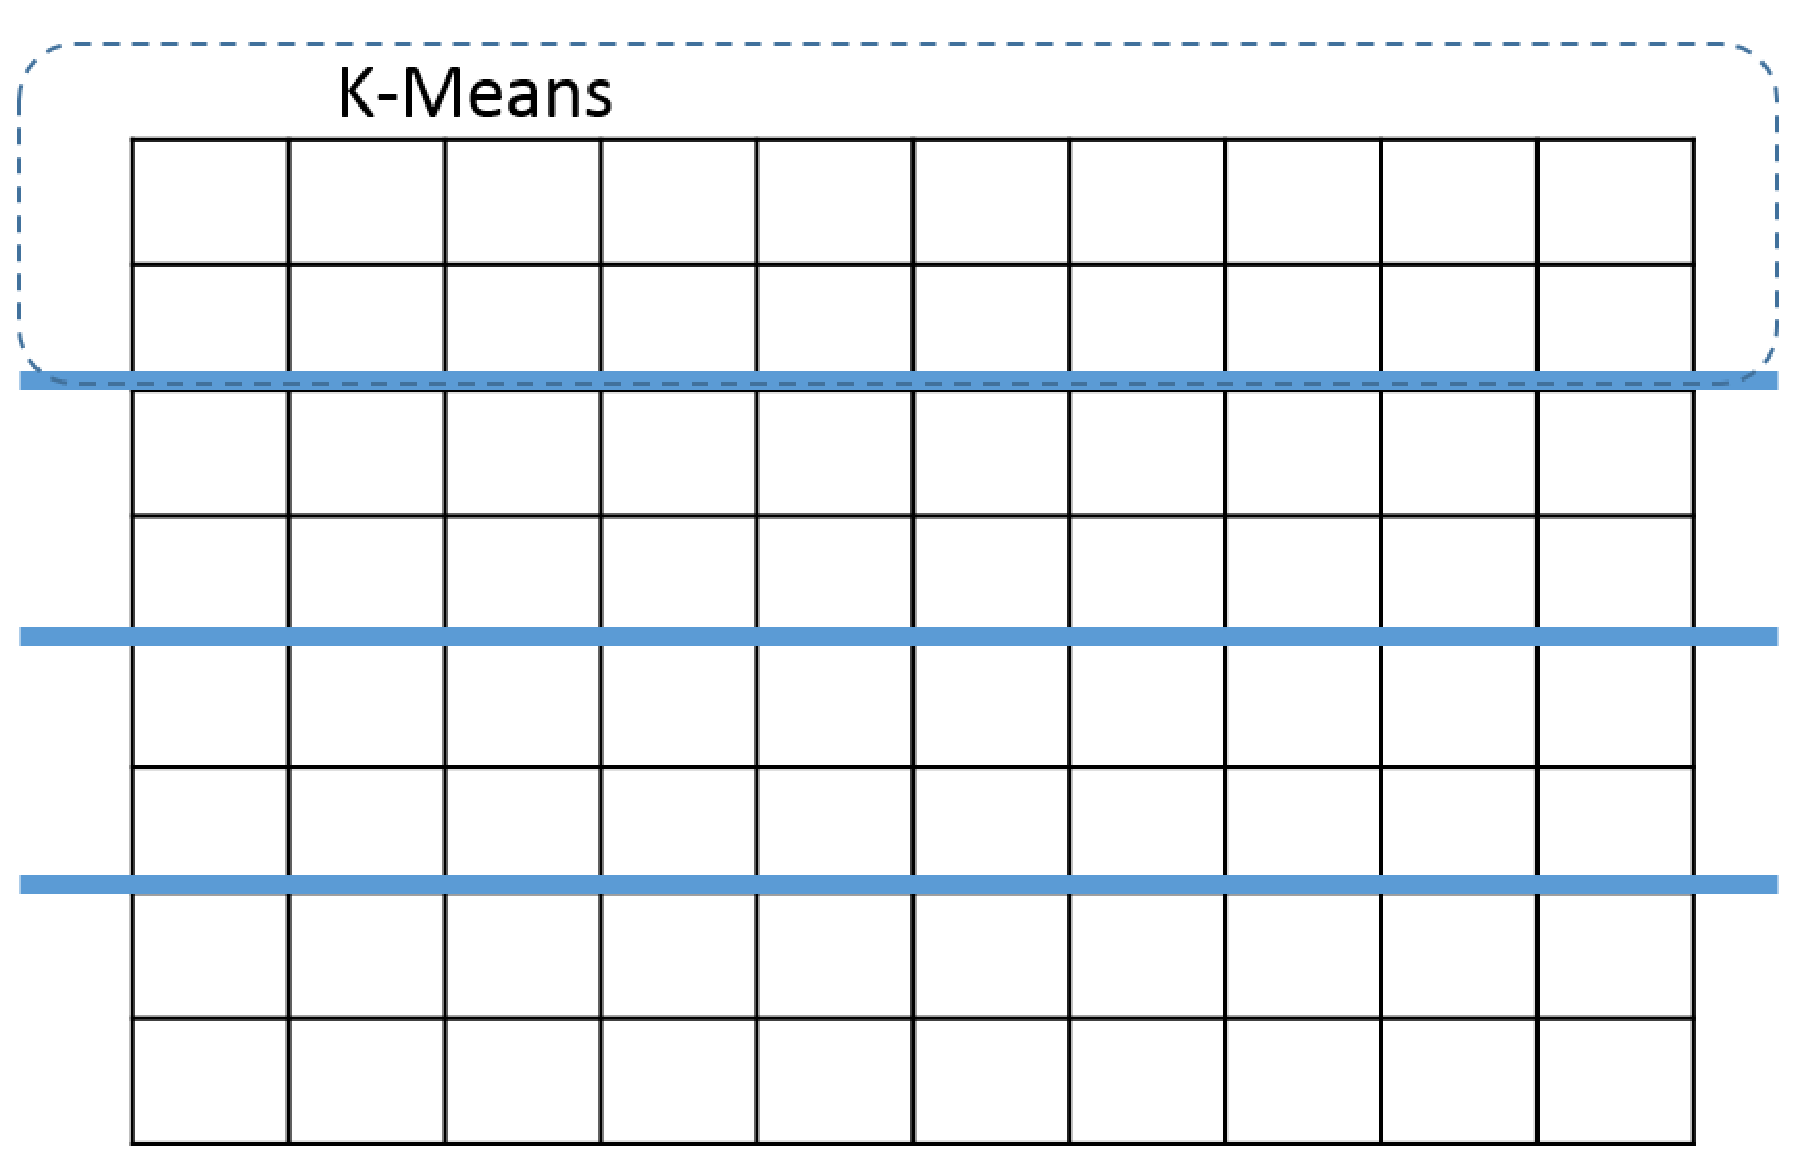
\includegraphics[width=0.5\linewidth]{PQ_subspace}
  \caption{PQ 算法中子空间的划分}
  \label{fig:PQ_subspace}
\end{figure}
更为一般来说,我们可以得到乘积量化方法的目标函数如下:
\begin{equation}
\mathit{l}_\mathrm{PQ} = \sum_{i=1}^n\min\Bigg\lVert \mathbf{x}_i - \begin{bmatrix}C^1\mathbf{b}^1_i\\\vdots\\C^m\mathbf{b}^m_i\end{bmatrix} \Bigg\rVert _2^2
\end{equation}
其中 $\mathbf{b}^j_i \in \{0,1\}^h$且$\lVert\mathbf{b}^j_i\rVert=1$,$j \in \{1,\cdots,m\}$。在上面式子中,$C^j(j\in \{1,\cdots,m\})$ 就是我们需要求解的矩阵,在编码过程中,我们称其作为码本(codebook)。求解过程其实并不复杂,正如前文提到,在每个子空间中做 K-Means 聚类就可以求解出码本,这样我们就可以利用码本对每个子空间中的子向量进行编码,从而对原始向量进行编码表示。
\section{利用乘积量化的近似近邻查询}
前文所提的乘积量化只是介绍了如何进行数据的压缩编码,那么乘积量化到底如何应用到近似近邻查询当中呢?
\section{Spark 上的分布式实现}
\subsection{RDD 的划分}
\subsection{训练阶段}
\subsection{编码阶段}
\subsection{查询阶段}

